\section{}
\label{sec:problem1}
%%%%%%%%%%%%%%%%%%%%%%%%%%%%%%%%%%%%%%%%%%%%%%%%%%%%%%%%%%%%%%%%%%%%%%
\paragraph{a)} Missing: relate cells and pines to nature.

For this task, three sets of real data points are studied. The data is loaded from the course web page.

\begin{figure}
    \centering
    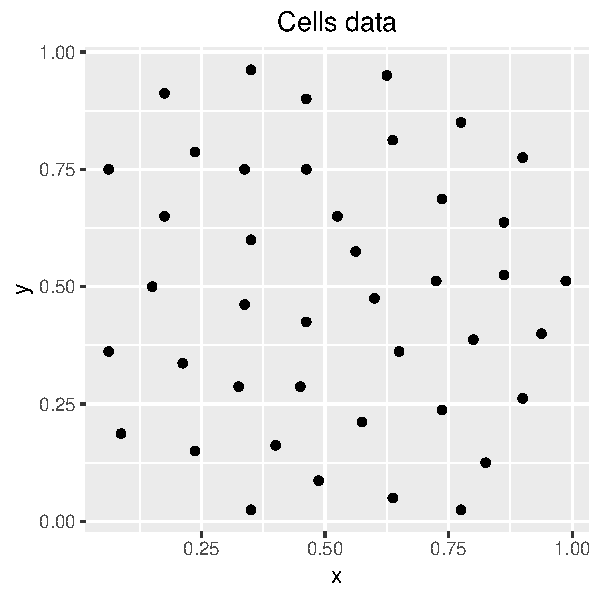
\includegraphics[scale=0.95]{figures/prob1_cells_points.pdf}
    \caption{Data points from \textit{cells.dat}}
    \label{fig:cells_points}
\end{figure}

\begin{figure}
    \centering
    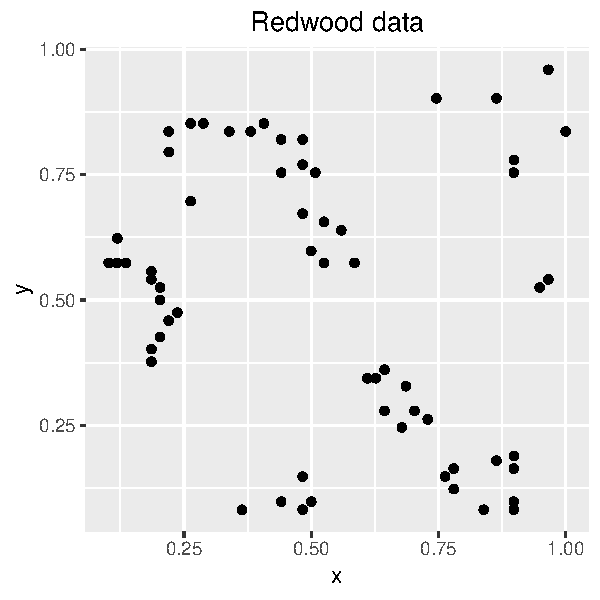
\includegraphics[scale=0.95]{figures/prob1_redwood_points.pdf}
    \caption{Data points from \textit{redwood.dat}}
    \label{fig:redwood_points}
\end{figure}

\begin{figure}
    \centering
    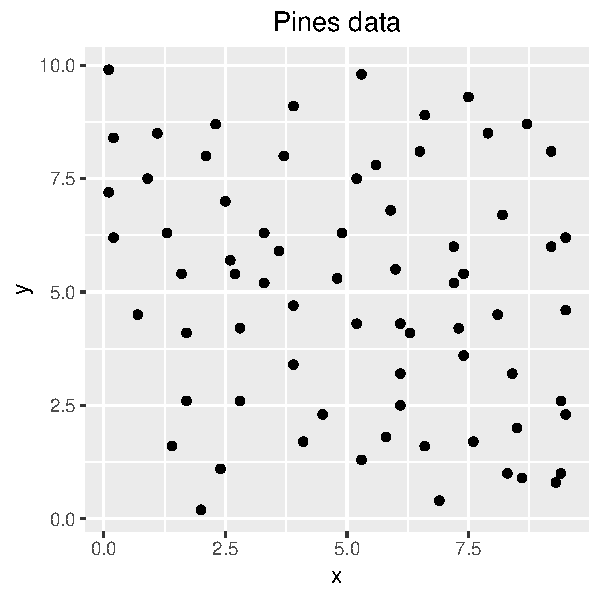
\includegraphics[scale=0.95]{figures/prob1_pines_points.pdf}
    \caption{Data points from \textit{pines.dat}}
    \label{fig:pines_points}
\end{figure}

Figures \ref{fig:cells_points}, \ref{fig:redwood_points} and \ref{fig:pines_points} show the three different data point patterns. These patterns have different properties. The pines data points in figure \ref{fig:pines_points} seem to be scattered around at random; some close together and some further away without any particular trend. The redwood data points (figure \ref{fig:redwood_points}) are more clustered. This is actually a known feature for redwood trees, as baby redwoods often grow on top of the roots of their parents to get nutrients (https://www.livescience.com/39461-sequoias-redwood-trees.html). The cells (figure \ref{fig:cells_points}) data on the other hand, show the exact opposite property. The points seem to be spread out to max out the space for each cell points, i.e. there seem to be a repulsive effect.

%%%%%%%%%%%%%%%%%%%%%%%%%%%%%%%%%%%%%%%%%%%%%%%%%%%%%%%%%%%%%%%%%%%%%%
\paragraph{b)}

$J(t)$ is an interaction function related to the distance from an event $\vect{x_0}$ to nearby events. Let $\textrm{B}_{x_0}(t)$ be the ball with center in $\vect{x_0}$ and radius $t \geq 0$. Then the number of events inside $\textrm{B}_{x_0}(t)$ is $k_{\textrm{B}_{x_0}(t)}$ and
\begin{equation}
    J(t) = \frac{\E{[k_{\textrm{B}_{x_0}(t)}-1]}}{|\textrm{B}_{x_0}(t) \cap \textrm{D}|}.
\end{equation}
The $-1$ corrects for the event $\vect{x_0}$ already known to be inside the ball. For a stationary Poisson Random Field, the expected number of events inside an subdomain of D is the intensity $\lambda_k$ times the area of the subdomain, since the intensity is constant over the whole domain. Thus, for a stationary Poisson RF, 
\begin{equation}
    J(t) = \frac{\lambda_k |\textrm{B}_{x_0}(t) \cap \textrm{D}|}{|\textrm{B}_{x_0}(t) \cap \textrm{D}|} = \lambda_k.
\end{equation}

Another alternative for evaluating the interaction is using the L-interactive function. For domains in $\R^2$, this is

\begin{equation}
    L(t) = \left[\frac{\E{[k_{\textrm{B}_{x_0}(t)}-1]}}{\lambda_k \pi}\right]^{1/2} = \left[\frac{J(t)|\textrm{B}_{x_0}(t) \cap \textrm{D}|}{\lambda_k \pi}\right]^{1/2}.
\end{equation}

Ignoring boundary effects, that is assuming $|\textrm{B}_{x_0}(t) \cap \textrm{D}| = |\textrm{B}_{x_0}(t)| = \pi t^2$, 
\begin{equation}
    L(t) = \left[\frac{J(t)\pi t^2}{\lambda_k \pi}\right]^{1/2} = \sqrt{\frac{J(t)}{\lambda_k}}t .
\end{equation}

Inserting for $J(t)$ we get that for stationary Poisson RF
\begin{equation}
    L(t) = t
\end{equation}

In R, the empirical L-interaction function can be found using the function Kfn() from the library \textit{spatial}. The empirical L-function for the three data sets are shown in figure \ref{fig:L_emp}. The plots follow more or less the same straight line for intermediate distances, but for large and in particular for small distances, the functions are somewhat different. The \textit{cells data} seem to have little interaction at small distances, but has the highest at large distances. The \textit{redwood data}, on the other hand, seem to have higher interaction at small distances. This fits with the observations from problem 1a) that the \textit{redwood data} seemed to be more clustered than the others and the \textit{cells data} more repulsive. 

\begin{figure}
    \centering
    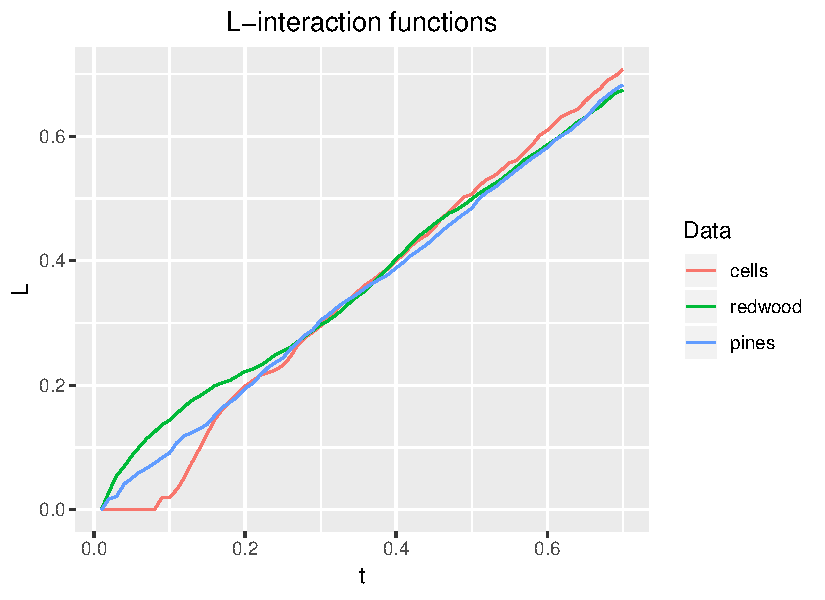
\includegraphics[scale=0.95]{figures/prob1_L_empirical.pdf}
    \caption{Empirical L-interaction functions for the three data sets.}
    \label{fig:L_emp}
\end{figure}

If a stationary Poisson RF is a good model for the data sets, then the empirical L-function should approximately follow $L(t) = t$. In figure \ref{fig:L_emp_theor}, the empirical interactive functions are plotted against this line. Here, deviation from the line at small distances for the \textit{cells data} and the \textit{redwood data} becomes maybe even more apparent. The \textit{pines data} follows the pretty well, though there is some deviation for larger distances. 

\begin{figure}
    \centering
    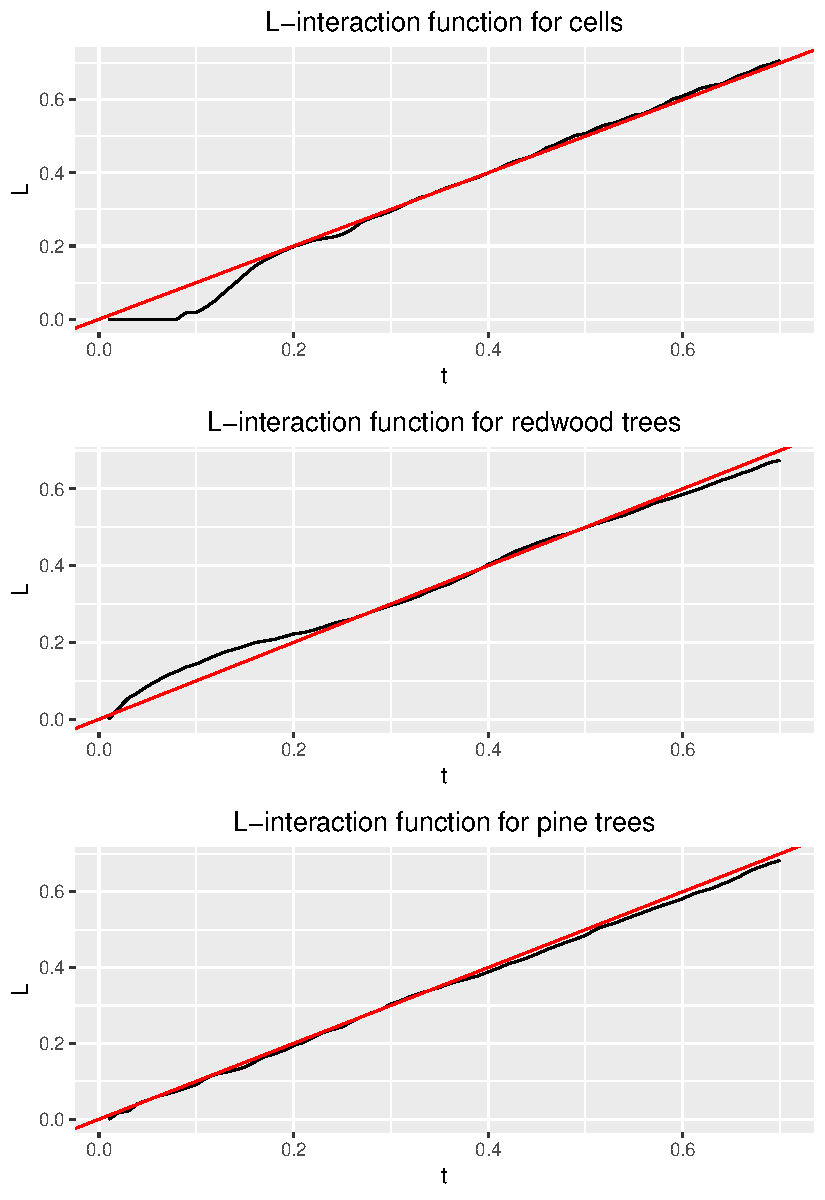
\includegraphics[scale=0.95]{figures/prob1_L_emp_theor.pdf}
    \caption{Empirical L-interaction functions for the three data sets (black lines) plotted against the theoretical (red lines). If a stationary Poisson RF is a suitable model, the red and black lines should more or less overlap.}
    \label{fig:L_emp_theor}
\end{figure}

It seems that a stationary Poisson model may be suitable for the pine tree data, but not for the two other data sets. The redwood data seem to be clustered and the cells data seem to be repulsive. However, empirical data must be expected to deviate somewhat from the theoretical value, and to make a more robust conclusion, a test will be performed.

%%%%%%%%%%%%%%%%%%%%%%%%%%%%%%%%%%%%%%%%%%%%%%%%%%%%%%%%%%%%%%%%%%%%%%
\paragraph{c)}
We will now perform an empirical Monte Carlo test to assess whether a stationary Poisson Random Field is a suitable model for each point pattern. Assuming that the data is indeed from a stationary Poisson RF, and conditioning on the number of events, the locations of each event is independent and uniformly distributed in the domain. 

The domain for each data set is the square $[0,1] \times [0,1]$, to generate realizations of the Poisson RF, we can draw $x$-coordinates and $y$-coordinates from a uniform (0,1)-distribution. For each data set we draw $100$ realizations with the same amount of data points as in the original set. That is, for the \textit{cells} data, which consists of $42$ points, we sample $42\cdot 100$ $x$-coordinates and the same amount of $y$-coordinates, uniformly. For each realization, we compute the empirical L-function, and then we use these to test whether the original data set may origin from a Poisson RF.


